\chapter{BACKGROUND}
    \section{Distributed machine learning and SGD}
    % \todo{Aritra: After you write it, I will work on this.}
    
    As we already discussed, inducing parallelism during the training phase of deep neural networks has become mandatory.
    Apart from exploiting the inherent parallelism of training computations by employing dataflow-graph representations and incorporating multi-threading mechanisms, there are also methods for distributing this computational workload in more than one nodes.
    A lesser known method is the so-called "model parallelism" approach
    which proposes the partition of the model to multiple workers.
    The model is one unique replica spanning across a number of different nodes that
    communicate with each other in order to send and receive tensors.
    Whereas most deep learning frameworks support this kind of partitioning and are equipped with some naive node-placement mechanisms that try to come up with ideal partitioning options, this method is not usually favored. Obtaining good partitions is often challenging and also, not all models benefit from this mode of execution on the first place.
    Data parallelism is a widely-known alternative approach which proposes the replication of the model in multiple workers. Those replicas will be trained separately on different partitions of the training dataset. 
    The local, intermediate gradients that are computed at each iteration of the backpropagation algorithm, will be exchanged between the workers and an aggregated version of them will be used for the update of the corresponding model-parameters.
    This process will be repeated for all the training epochs.
    
    The backpropagation algorithm that generates those gradients is typically an instantiation of the Stochastic Gradient Descent (SGD) optimizer \cite{robbins1951}.
    SGD is a variation of the gradient descent method and computes the gradients from arbitrarily selected subsets of the dataset instead of the entire portion of it.
    Those gradients, thereby, are considered to be stochastic approximations of the actual ones and they are significantly easier to calculate.
    
    \section{Compressed communication \cite{10754/662495}}
    
    The gradient exchange between workers through the network creates a bottleneck for the overall training. 
    Compressed communication aims to alleviate this issue by introducing lossy compression on the transferred data.
    The stochastic nature of training, induced by the selection of the SGD optimizer, allows the model to converge despite the small loss of gradients information.
    This has enabled the emergence of various compression methods all of whom can be classified in the following categories:
    
    \begin{itemize}
        \item {\bf Quantization Methods} reduce the size of the gradient by diminishing the number of bits needed to represent the gradient components. 
        For example, a "float-16" compression method receives a tensor of type "float-32" and converts it to "float-16", representing this way each gradient component using 16 fewer bits.
        
        \item {\bf Sparsification Methods} aim to encode the gradient by converting it to a sparsed tensor. Those methods choose to keep only a subset of the gradient components as well as their respective positions in the initial tensor. For example, Top-r keeps only the top $r$ absolute components of the gradient whereas Random-r keeps only $r$ randomly selected values.
        
        \item { \bf Low-Rank Methods} decompose the gradient tensor into low rank matrices. 
        That is, matrices that require less space for their storage.
         
    \end{itemize}
 
    There are also {\bf hybrid methods} which are combinations of the above but discussing them would be outside the scope of this work.
    
    \subsection{Sparsification Methods}
    This family of compression methods is essential for our work, therefore, it is mandatory to elaborate more on it.
    Following the formalization proposed in \cite{10754/662495},
    let $g$ be a stochastic gradient of size $N$ that we want to compress and let $b$ be a bitmask vector thas has the same size.
    Every bit $b[i]$ inside the bitmask is then set to either $1$ or $0$ depending on whether the corresponding value of $g$ in position $i$ is selected by the sparsification method or not.
    The element-wise product of $b$ and $g$ is the sparsified tensor and can be represented in various ways.
    The simplest representation would be to use two separate vectors, one for the selected gradient components and one for their corresponding positions, also known as indices. Note that, the indices are the positions in $b$ that have a $1$ bit-value.
    \begin{itemize}
        \item In {\bf Top-r} sparsification method \cite{Aji_2017}, \cite{alistarh2018convergence}, we select a bitmask $b$ so that for every $b[i]=1$ we have that $g[i]$ is a value that belongs in the set of top $r$ largest absolute values of $g$.
        
        \item In {\bf Random-r} sparsification method we select randomly a subset of $r$ indices for which the corresponding values in the bitmask are all set to 1.

    \end{itemize}
    Both Top-r and Random-r are fixed-dimension sparsification methods since the sizes of the encoded tensors that they yield are fixed and controlled by $r$.
    Now, $r$ can be either hard-coded and explicitly specified by the user or can be defined implicitly by the "compress ratio" parameter. This is usually a percentage that indicates how sparse we want the gradient to become after compression. For example, if the initial gradient has a size of 100 values then a compress ratio of 0.1 would set the $r$ equal to 10. 
    
    
    \subsection{Memory Compensation}
    Memory Compensation is a mechanism that compensates for errors accumulated due to the lossy nature of most compression methods \cite{stich2018sparsified}.
    We keep track of those errors and accumulate them in a memory vector $m$ which we update right after the compression of a gradient takes place with the following rule: 
    
    \begin{flushleft}
    \centering
    \setlength{\parindent}{40ex} 
    $m_{t+1} := m_{t} + g_{t} - compression(g_{t})$
    \end{flushleft}
    
    Then, we compensate for these errors by updating the gradient of the next iteration as follows:
    \begin{flushleft}
    \centering
    \setlength{\parindent}{40ex} 
    $g_{t} := \beta m_{t} + \gamma g_{t}$
    \end{flushleft}
    where $\beta>0$ is the memory decay factor and $\gamma>0$ weighs the relevance of the latest stochastic gradient.
    
    
    \newpage
    
    \section{Bit compression}
    Every kind of information is represented in machines as a stream of bits.
    Reducing the size of those streams by compressing them is highly desired in many applications. 
    There exist various bit-level methods for encoding these raw sequences of ones and zeros and they are classified as either lossless or lossy.
    We call lossless those compression methods that yield encodings which we can precisely decode without losing any part of the initial information. On the contrary, lossy methods allow some loss of information.
    
    \subsection{Run length encoding}
    Run Length Encoding is a very simple and popular bit-level compression method that replaces sequences of continues ones or zeros with integers representing their lengths \cite{rle}. 
    Note that, those integers are represented in an efficient way.
    For example, a common 32/64-bit integer representation may not be good in cases where the lengths are small as it would consume much more space than the one actually needed.
    Instead, code-blocks of user-defined size are used depending on the characteristics of the given bit-stream.
    
    This encoding method is inefficient when the ones and zeros are uniformly distributed inside the bit-streams. On the contrary, when there are large and continuous repetitions of the same bits in the stream this method performs well. 
    
    For example, consider the following bit-streams, A and B:
    
    \begin{itemize}
        \item {\bf Bit-stream A:} $[0,1,1,0,0,1,0,1,0,0,0,1,1]$, {\bf Lengths:} $[1,2,2,1,1,1,3,2]$
        \item {\bf RLE using 2-bits per integer:} $[0,1, 1,0, 1,0, 0,1, 0,1, 0,1, 1,1, 1,0]$
        \item {\bf Bit-stream B:} $[0,0,0,0,0,0,1,1,1,1,1,1,1]$, {\bf Lengths:} $[6,7]$
        \item {\bf RLE using 3-bits per integer:} $[1,1,0, 1,1,1]$
    \end{itemize}
    
    Note that, for each case we used the ideal size of code-blocks for representing the integers.
    Still, the encoding of A has a size of 16 which is larger than the size of the initial bit-stream representation.
    In the second case, however, we have a gain of 7 bits.
    
    \begin{figure}[h]
    \centering
    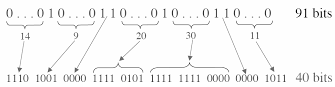
\includegraphics[scale=1]{thesis/figures/rle.png}
    \caption{Run Length Encoding of a bit-stream, counting only the zeros}
    \label{rle}
    \end{figure}
    
    Run Length Encoding has itself a lot of variations. 
    For example, one could count only the zeros and not the ones, as shown in figure \ref{rle}, or vice versa. In this figure, we are counting only the continuous zero-bits. When two continuous one-bits occur, then we imply that a zero-bit sequence of length zero exists between them.
    
    We have created a variety of RLE implementations that we use as baselines for evaluating our own bloom filter method, as we will discuss in the evaluation section. 
    
    \newpage
    \subsection{Bloom Filters}
        Bloom Filters are the most common and widely-known probabilistic data structures.
        They belong in the greater family of Approximate Membership Query Data structures (AMQ) and provide probabilistic answers about whether an element exists in a
        particular set or not.
        They are usually stored in memory and their tremendous space-efficiency properties have made them extremely popular for a variety of applications.
        One common use-case for bloom filters is when we want to avoid searching slow-mediums (e.g. hard disks) for records that are not actually stored there.
        
        When a bloom filter is queried for a given element, it can return either a definitely negative answer or a positive one with some degree of uncertainty.
        Any non-negative answer is usually assumed by the user as a positive one, however,
        there is no guarantee that the answer is not actually negative.
        This gives birth to the popular false positive rate (FPR) metric that is used for evaluating the performance of those filters, as it measures the probability that they provide a false-positive answer.
        
        AMQ data structures have been studied extensively since their conception and more sophisticated versions of them are continuously developed.
        We continue by providing a  more formal description of what they are and how they operate.
        % We will mention some of the most interesting variations of bloom filters, 
        % but first, we must provide a more formal description of what they are and how they operate.
        
        \begin{figure}[h]
        \centering
        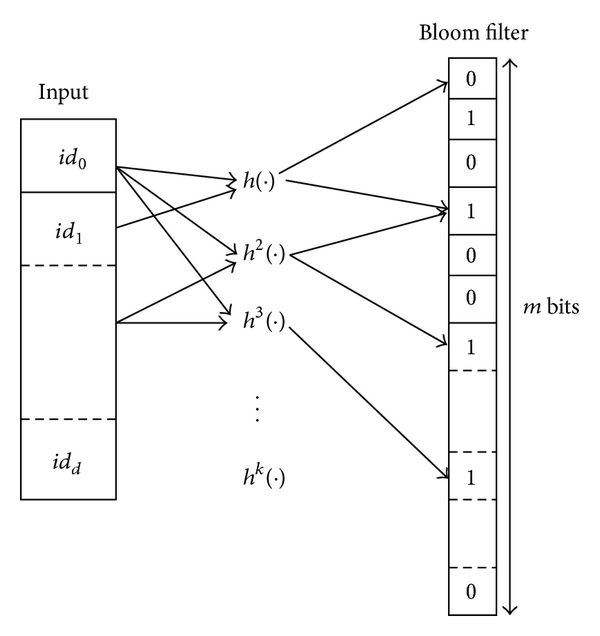
\includegraphics[scale=1.7]{figures/bloom_filter.jpg}
        \caption{Bloom Filter}
        \end{figure}
        
        A bloom filter $\cB$ is commonly an array of $m$ bits that is built on the $r$ elements of the set $S = \{x_1,x_2,\cdots\,x_r\}$ that we wish to represent.
        At construction phase, all bits are initialized to zero. 
        We insert every element of $S$ in the array by using $k$ hash functions, all independent to each other. Every hash function maps an item $x \in S$ to a position inside the bloom filter. The bit that corresponds to every such position is then set to one. 
        Consequently, every insertion of an element $x \in S$ inside the bloom filter causes a side effect to at most $k$ different bits.
        Note that, in practice, only the first bit-change at each location has effect. That is, if a bit-location is already set to 1 from a previous hashing, any other changes at that bit-location due to consequent hashing have no effect.
        
        \begin{figure}
        \centering
        \begin{minipage}{0.7\textwidth}
        \begin{algorithm}[H]
        	\SetAlgoLined
         	\SetKwInOut{Input}{Input}
        	\SetKwInOut{Output}{Output}
             \SetKwInOut{Init}{Initialize}
             \SetKwInOut{Compute}{Compute}
        \nl\Input{Bloom Filter $\cB$ with $m$ bits all set to 0,\\
                $k$-hash functions $h_i$, \\a set of $r$ elements $S$\;}
        \nl \For{each $x_i\in S$}
        	{ \nl \For{$j = 1,2,\cdots, k$}
        		{  \nl  Set the bit in location $h_j(x_i)$  to 1;
        		}
         	}
         	\nl \Output{A Bloom filter $\cB$.}
         	\caption{Building a Bloom Filter on the set $S$ } \label{alg_1:build_BF}
        \end{algorithm}
        \end{minipage}
        \end{figure}
        
        \hskip .6cm
        
        \begin{figure}
        \centering
        \begin{minipage}{0.7\textwidth}
        \begin{algorithm}[H]
        	\SetAlgoLined
         	\SetKwInOut{Input}{Input}
        	\SetKwInOut{Output}{Output}
             \SetKwInOut{Init}{Initialize}
             \SetKwInOut{Compute}{Compute}
        \nl\Input{Bloom filter $\cB$, $k$-hash functions $h_i$, an element $x$\;}
        	{\nl \For{$i = 1,2,\cdots, k$}
        	{\nl Use hash function $h_i$ on $x$\;
        		\nl \If{$h_i(x)=0$ for any $i$}
        		    {\nl $x\notin S$ and {\tt Break}\;
                \ElseIf{$h_i(x)=1$ for all $i$}
        		    {\nl $x$ may or may not be in $S$\;}
                    }
        	}
         	}
         	\caption{Querying an element by using Bloom filter} \label{alg_1:query_BF}
         \end{algorithm}
        \end{minipage}
        \end{figure}


        Once the filter is constructed, we say that it represents the set $S$ in the sense that it can provide probabilistic answers about whether an element exists in $S$ or not. For querying an element $x \in S$ we must pass it through the $k$ different hash functions and check the value of the bits in the corresponding positions. If at least one bit is set to zero then the filter returns a negative response and we definitely know that $x$ does not belong in $S$. 
        Otherwise, $x$ may or may not belong in $S$.

        The process for building a bloom filter on a set $S$ or querying an element using the bloom filter is described in Algorithms \ref{alg_1:build_BF} and \ref{alg_1:query_BF}, respectively.
        

    \subsubsection{Bloom Filter Specifications}

    \cite{5751342} Given $m$ the size of the bloom filter and $r$ the number of items inserted in it, the number of hash functions that minimizes the probability of false positives is computed as:
    $k=\frac{m}{r}\log 2.$ 
    This $k$ results in the probability of false positive, $\epsilon$ as: $\log\epsilon=-\frac{m}{r}(\log 2)^2.$ 
    In practice, we need to calculate the bits in the filter by using the relation $m=\frac{-r\log\epsilon}{(\log 2)^2}$ and the number of hash functions by $k=\frac{-\log\epsilon}{\log 2}$.

    \newpage

    \section{Curve Fitting}
    % \todo{Aritra: Great! I would like to make a pass once you are done}
    
    Regression is considered to be a large sub-category of supervised learning.
    Curve fitting, which is an example of regression, is the process of constructing a curve that can fit to a series of data points in an N-dimensional space.
    This curve is defined by a mathematical function that our goal is to specify.
    Curve fitting can be categorized as either interpolation  or smoothing depending on whether we wish to create a curve that precisely fits the data or simply approximates it.
    It is common to assume that the function has a specific parametric form 
    and then try to estimate the unknown coefficients that fully define the curve.
    
    In figure \ref{curve_fit}, we have a set of points $(x_n, y_n), n=1,2\dots,N$ that lie in the $\mathbb{R}^2$ space
    and we adopt the following parametric functional form: $y=a+bx$, which denotes a simple, straight line.
    
    In order to measure how well the curve matches the data points we can employ a variety of  
    loss functions.
    The loss function commonly quantifies the deviation between the estimated values of $y$ and the true $y$ values (ground truth).
    This deviation is also called "error" and we ideally want to minimize it as much as possible.
    
    
    \begin{figure}[h]
    \centering
    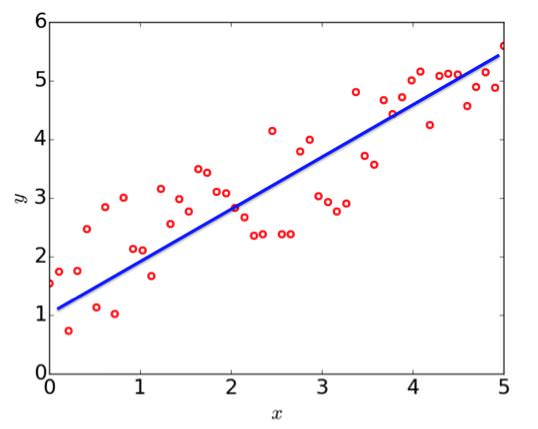
\includegraphics[scale=0.5]{thesis/figures/curve-fitting.jpg}
    \caption{Curve Fitting}
    \label{curve_fit}
    \end{figure}
    
    One example is the Least Squares (LS) loss function which is defined as follows:
    \begin{flushleft}
    \centering
    \setlength{\parindent}{40ex} 
    $\mathcal{L}(a,b) = \sum_{n=1}^N (y_n-f_{a,b}(x_n))^2$
    \end{flushleft}

    and measures the sum of the squared distances between the true values and the estimated ones.
    The straight-line regression is one of the simplest regression models, however, many more exist.
    We characterize regression as linear or non-linear depending on whether the model is linear in the coefficients or not.
    We can employ more complex, non-linear parametric functional forms in order to capture 
    non-linear, curved relationships between the dependent variable $Y$, and one or more independent variables $X$
    and we can also apply a variety of different loss functions, every one of them leading to a different optimization problem and thus,
    different techniques for finding the optimal coefficients.
    
    As we will discuss, curve fitting is used in our setting for compressing the values of the gradient components, however, a more extended analysis of the theory behind regression would be outside the scope of this thesis.
    
    